\documentclass[10pt,letterpaper]{article}
\usepackage[top=0.85in,left=2.75in,footskip=0.75in,marginparwidth=2in]{geometry}

% use Unicode characters - try changing the option if you run into troubles with special characters (e.g. umlauts)
\usepackage[utf8]{inputenc}

% clean citations
\usepackage{cite}

% hyperref makes references clicky. use \url{www.example.com} or \href{www.example.com}{description} to add a clicky url
\usepackage{nameref,hyperref}

% line numbers
\usepackage[right]{lineno}

% improves typesetting in LaTeX
\usepackage{microtype}
\DisableLigatures[f]{encoding = *, family = * }

% text layout - change as needed
\raggedright
\setlength{\parindent}{0.5cm}
\textwidth 5.25in 
\textheight 8.75in

% Remove % for double line spacing
%\usepackage{setspace} 
%\doublespacing

% use adjustwidth environment to exceed text width (see examples in text)
\usepackage{changepage}

% adjust caption style
\usepackage[aboveskip=1pt,labelfont=bf,labelsep=period,singlelinecheck=off]{caption}

% remove brackets from references
\makeatletter
\renewcommand{\@biblabel}[1]{\quad#1.}
\makeatother

% headrule, footrule and page numbers
\usepackage{lastpage,fancyhdr,graphicx}
\usepackage{epstopdf}
\pagestyle{myheadings}
\pagestyle{fancy}
\fancyhf{}
\rfoot{\thepage/\pageref{LastPage}}
\renewcommand{\footrule}{\hrule height 2pt \vspace{2mm}}
\fancyheadoffset[L]{2.25in}
\fancyfootoffset[L]{2.25in}

% use \textcolor{color}{text} for colored text (e.g. highlight to-do areas)
\usepackage{color}

% define custom colors (this one is for figure captions)
\definecolor{Gray}{gray}{.25}

% this is required to include graphics
\usepackage{graphicx}

% use if you want to put caption to the side of the figure - see example in text
\usepackage{sidecap}

% use for have text wrap around figures
\usepackage{wrapfig}
\usepackage[pscoord]{eso-pic}
\usepackage[fulladjust]{marginnote}
\reversemarginpar

% document begins here
\begin{document}
\vspace*{0.35in}

% title goes here:
\begin{flushleft}
{\Large
\textbf\newline{Domestication lead to a drastic reduction of core-genome in the two lineages of domesticated rices}
}
\newline
% authors go here:
\\
Cécile Monat\textsuperscript{1,2{+}\textdagger},
Nguyet Dang\textsuperscript{1,2\textdagger},
Christine Tranchant-Dubreuil\textsuperscript{1,2\textdagger},
Stefan Engelen\textsuperscript{3},
Karine Labadie\textsuperscript{3},
Patrick Wincker\textsuperscript{3},
Ndomassi Tando\textsuperscript{1,2},
Emmanuel Paradis\textsuperscript{4,5},
and François Sabot\textsuperscript{1,2*}
\\
\bigskip
\bf{1} DIADE, Univ of Montpellier, IRD, Montpellier, France
\\
\bf{2} South Green Bioinformatics Platform, IRD, BIOVERSITY,CIRAD,INRA, Montpellier, France
\\
\bf{3} CEA, Genoscope, Evry, France
\\
\bf{4} ISE-M, Univ of Montpellier, CNRS, IRD, EPHE, Montpellier, France
\\
\bigskip
* Corresponding author: francois.sabot@ird.fr\\
{+} Present address: Leibniz Institute of Plant Genetics and Crop Plant Research (IPK) Gatersleben, Seeland, Germany\\
\textdagger Those three authors contribute equally to the work\\
\end{flushleft}

\section*{Abstract}
% %Fitting multiple figures into very tight manuscripts while keeping it pleasant to read is challenging. Therefore figures are often simply attached to the very end of a manuscript file. While easier for the authors, this practice is inconvenient for readers. This \LaTeX template shows how to generate a compiled PDF with figures embedded into the text. It provides several examples of how to embed figures or tables directly into the text thus giving you a range of options from which you should choose the one best suited for your manuscript. Check out Schlegel et al., (2016) as example of use \cite{Schlegel2016}.
% Pangenome theory implies that individuals from a given group/species share only a given part of their genome (core-genome), the remaining part being the dispensable one. Domestication process implies a small number of founder individuals, and thus a large core-genome compared to dispensable at the first steps of domestication. We sequenced at high depth 120 cultivated African rice \textit{Oryza glaberrima} and of 74 wild relatives \textit{O. barthii}, and mapped them on the external reference from Asian rice \textit{O. sativa}. We then use a novel DepthOfCoverage approach to identify missing genes. After comparing the two species, we shown that the cultivated species has an unexpectedly smaller core-genome than the wild one, as well as an expected smaller dispensable one. Those findings replace in perspective the inadequacy of cultivated crops to wilderness and their lack of resilience in challenging context.
% now start line numbers
\linenumbers

% the * after section prevents numbering
\section*{Introduction}
Doemstication of rices occured independantly...
Diversity loss/founder effect/genetic drift....
However, most previous analyses of domestication impact on diversity were limited to few markers or SNP-based. Recent papers \cite{REFpangenome} shown that the diversity is not only linked to the SNP and short InDels, but also to Presence/Absence Variations (PAV) and Copy Number Variation (CNV). This lead to the idea of Pangenome \cite{Tettelin2005, Tranchant2018}, composed of the core genome, genomic sequences shared between all individuals of the considered group, and of the dispensable genome, genomic sequences shared between some individuals (or even only one) but not all. Currently, only a few studies focused on the pangenome of plants, and only one, to our knowledge \cite{Han2018}....

In this paper, we benefit of the release of very large scale data on the two domesticated rice species, the Asian rice \textit{Oryza sativa} \cite{3krgp} and the African one \textit{O. glaberrima} \cite{Cubry2018}, and on their respective wild relatives, \textit{O. rufipogon} (this paper) and \textit{O. barthii} \cite{Cubry2018}, to explore the impact of domestication on the core genome of cultivated.
% Pangenome \cite{Tettelin2005,Tranchant2018} is defined as the whole set of DNA sequence present in a given group (such as a species). This pangenome is further divided in three compartments:(\textit{i}) the core-genome, composed of sequences present in all individuals of the group; (\textit{ii}) the dispensable/variable/accessory-genome, sequences present in some but not all of the individuals; and (\textit{iii}) the individual-specific genome, accounting for sequences present only in a single individual of the group. It has been first defined on microorganism \cite{Tettelin2005} and is now commonly used on bacteria with some specifics tools developed for this type of analysis \cite{Laing2010, Snipen2010, Zhao2012,Sarovich2014, Hennig2015, Thakur2016}. Few studies also started on other genera like animals \cite{Boussaha2015}, Human \cite{Li2010}, viruses \cite{Aherfi2014}, algae \cite{Wang2014a}, fungi \cite{Upadhyaya2015} and plants \cite{Cheung2009, Yao2010, Montenegro2017}.
% 
% From this comes the idea that each individual has differences not only in term of alleles but also in term of sequence numbers and composition \cite{Chia2012, Hennig2015, Lu2015}. Moreover two genomes are similar not only by the sequences which they share, but also because they miss the same sequences \cite{Snipen2010}. These type of studies also confirm that having a single reference genome per species is certainly helping but is not enough to represent the whole genomic diversity of a species, as the reference genome has sequences absent in other individual of the same species and miss some other ones \cite{Weigel2009, Gan2011, Upadhyaya2015}. 
% 
% %Manque une partie sur les impacts potentiels des diff génomiques, eg la stérilité, les anomalies de recombinaisons, les vigueurs hybrides, tout ca
% Pan-genomic is thus a new way to understand evolution processes (such as sympatric speciation), and to establish new link between individuals (for instance, the link between two sub-species) as well as between different species. 
% 
% %Petit texte à ajouter sur la domestication ici
% One interesting aspect is to better characterize and understand the domestication process and its effects on genome, especially on genome diversity and structure.\\
% 
% Several studies showed that the analysis of several genomes belonging to the same species allowed to discover more intra-species diversity than expected \cite{Tettelin2008}. Therefore, doing comparative genomics of pan-genomic type put forward the interest to work within the same species to represent a diversity which would not be necessarily visible by looking only at the inter-species level \cite{Lukjancenko2012}. \\
% 
% Rice is the most cultivated cereal for human consumption, with two species cultivated, the Asian rice \emph{Oryza~sativa}, worldwide used, and the African rice \emph{Oryza~glaberrima}, endemic to West
% Africa. The latter and its wild relative \emph{Oryza~barthii} are known to have a very low diversity (SNPs based)\cite{Nabholz2014a} compared to other grasses. This characteristic makes them good models to study the genomic diversity in light of pan-genome as with a reasonable number of individuals will cover the entire diversity of the species. For that purpose we resequenced 194 accessions of African rices (120 of the cultivated species and 74 of its wild relative) with Illumina technology and shown huge genic variations during domestication.\\

\section*{Materials and Methods}

 \subsection*{Plant material}
  One hundred and eighty-two accessions of \emph{Oryza~glaberrima} and 82 accessions of \emph{Oryza~barthii} were used in the study (see \texttt{annexe E}) and described in \cite{Cubry2018} (Supplementary Data S1). For Asian rices, we selected 450 samples from the 3,000 Rice Genome Project (3kRGP, \cite{3kRGP}) based on their location on the global diversity and their high-level of data (min 20x, Supplementary Data S1), and obtained 45 \textit{O. rufipogon} sequences in Illumina, high-depth by Genocsope through the IRIGIN project (\url{http://irigin.org}). 
  
  \subsection*{DNA Sequencing}
  DNA was sequenced at the Genoscope (Evry, France) on Illumina HiSeq 2000/2500/400 with paired-end reads, 100 bases long, and cleaned as described in \cite{Cubry2018, Djedatin2017}. Briefly, the mean sequencing depth is of 35x with a maximum of 60x and a minimum of 20x, representing a total of XXXX and XXXX reads for \textit{O. glaberrima} and \textit{O. barthii}, respectively.

  \subsection*{Short reads mapping}
Cleaned reads were then mapped against the Asian reference genome (Os-Nipponbare-Reference-IRGSP-1.0/MSU7.0 \cite{Mcnally2009, Kawahara2013}) through a dedicated TOGGLe pipeline \cite{Monat2015, Tranchant2018}, as follows:
  FASTQC control, CutAdapt for removeing low-quality reads, repairing step to mate pairs, mapping with BWA aln/sampe legacy \cite{Li2009} (edit distance of 5 bases), conversion into BAM file with Picardtools (!!REF!!), extraction of properly and unproperly mapped in pair data with SAMtools \cite{Li2009a}. Properly mapped in pair reads were subject to  local realignment using GATK \cite{McKenna2010a}, duplicates removed with Picardtools (for details information about mapping see Supplementary Data S3).
  
  
  \subsection*{Reads count and normalization}
  % A revoir comme on lance sur pas mal de données différentes
  The reads count for each individual on 10kb bin (38,000 for a roughly 380Mb genome) were generated with the multicov tool from BEDTOOLS \cite{Quinlan2014}. Counts were normalized to 1 million total reads according to the initial individual sequencing coverage to obtain FP10KM values (Features per 10 kilobase per millions of reads).
  
  
  \subsection*{Pnorm and FDR analysis}
  Pnorm analysis and FDR approach at 5\% were performed using R and specific packages pnorm and qvalue \cite{Storey2015}. Annotations or bins for which the normalized reads count mean were lower than 2 were arbitrarily previously ride out the analysis and considered as absent for all individuals. Pan-matrix obtained shown '0' when gene/bin was considered as absent,  '1' if the gene/bin was considered as present and  'Uk' (Unknown) if feature does not pass the initial pnorm test.
  
  \subsection*{GO enrichment analyses}
  Genes underlying the PAV were recovered using the annotation v7 of the MSU7/IRGP1.0 assembly (\url{http://rice.plantbiology.msu.edu/})). Gene ontology enrichment analyses were performed using a home-made R script and the topGO package \cite{Alexa2016}, with a display of the 5 top most significant GO retrieved using the Fisher classic and weight01 algorithms.
  
  \subsection*{Identification of domesticated related gene families}
  GenFam was used...
  Data from gene families were obtained from Green Phyl V.4  \cite{Conte2008b, Conte2008a, Rouard2011}, selecting sequences without spliced forms.
  
  \subsection*{Availability of scripts}
  The whole bash, Perl and R scripts are available on github under Cecill-B/GPLv3 double licenses on the GitHub of the project: \url{HTTP}

\section*{Results}
\subsection*{Mapping and Normalization}
After cleaning, the raws reads were mapped against the Asian reference genome (Os-Nipponbare-Reference-IRGSP-1.0 \cite{Mcnally2009, Kawahara2013}). For African rices, we used 163 accessions of the cultivated African rice \textit{O.~glaberrima} and 86 accessions of its wild relative \textit{O.~barthii}, with a mean percentage of mapping of 86.49\% and 86.44\%, respectively \cite{Cubry2018}. For Asian rice, we used 3,000 library representing 450 samples representing rice diversity for the cultivated, with a mean value of xx\% of mapping, and 45 \textit{O. rufipogon} whole genome sequences. From these last samples, 3 of them harboured a very lower level of mapping compared to the other samples (less than 80\% compared to a minimum of 85\%); after careful check, they were removed as being not \textit{O.rufipogon} but \textit{O. meridionalis} and selected by error, ending up with 42 samples. We then performed reads count normalization according to the initial reads number specific to each individual reported to 1 million and the bin length, obtaining numerical F10KPM data. Distribution of F10PKM density mainly follows a normal law (see \texttt{Fig.\ref{distri}} for an example), thus we successively applied pnorm and FDR statisticals test to define if a given bin was present or not for each individual.

\subsection*{Chromosomal, individual and population effects}
We checked whether the global FP10KM profile were the same between the different chromosomes, between sequence type (gene, CDS, UTR or TE features) and if there were or not individual(s) effects. We seen that there are no significant differences between the 12 chromosomes on all the four groups analyzed (Supplementary Data S4).
We then performed the same analysis only on features representing exons (Supplementary Data 4) and representing not exons (\texttt{see Figs.~\ref{SeuilsNE_OG} and \ref{SeuilsNE_OB}}) and confirm profils are the same no matter the type of annotation features we are looking at. As a proxy for the rest of the chromosome we choose the chromosome 10 for the following verifications (central in the little range of chromosomes profiles).

In order to test if there were individual effect, we performed a hundred bootstrap-like analysis choosing 76 individuals.
No individual effect were detectable on \emph{O.~glaberrima} (\texttt{see Fig. \ref{BootstrapOG}}) but in \emph{O.~barthii} we found two classes of profils depending on the individuals in the group 
(\texttt{see Fig. \ref{BootstrapOB}}).
As described by Orjuela et al \cite{Orjuela2014}, this species can be divided in two populations respectively with 23 and 51 individuals distributed as in \texttt{Fig. \ref{SSpopOB}}.
To check if the two profiles were due to population split, we tested the hundred bootstrap analysis on \emph{O.~barthii} with only 23 individuals of the first population (\texttt{see Fig. \ref{BootstrapPOP1}}) 
and 51 of the second (\texttt{see Fig. \ref{BootstrapPOP2}}).
Two profiles were still detectable on the population 1, so we checked if 23 individuals was enough to determine these profiles. We performed the same analysis, only with the population 2 individuals but
with bootstrap of 23 individuals. This time the curves show more discrepancy suggesting that 23 is not a sufficient number of individuals to see a robust profile (\texttt{see Fig. \ref{BootstrapPOP2bis}}).
To be sure that it is necessary to have a minimum number of individuals to have a strong signal, we performed verifications on \emph{O.~glaberrima}. Both the 23 and 51 verifications conserved the robust profil 
(\texttt{see Figs. \ref{BGLAB51} and \ref{BootstrapGLAB23}}).

\subsection{Pan-genome compartments}
The pan-genome of \emph{O.~glaberrima} is comprised into the core-genome of \emph{O.~barthii} as it represents 39,106 and 39,730 genes respectively (see \texttt{Fig.~\ref{panGSize}}). On the other hand, the dispensable-genome of the cultivated species is bigger than wild one as its represents 5,299 and 745 genes respectively (see \texttt{Fig.~\ref{panGSize}, Table \ref{panG-glab} and Table \ref{panG-bar}}).
We identified 5,258 genes (more than 10\% of the repertoire of wild genes) common to the core-genome of \emph{O.~barthii} and to the dispensable-genome of \emph{O.~glaberrima}.  On the other hand we found only 23 genes common to the dispensable-genome of the wild species and the core-genome of the cultivated one. We were not able to detect any individual-specific genes.

We looked to the distribution of genes compartment along the chromosomes as presented in \texttt{Fig.~\ref{repartition}}. As expected the profile for the core and the dispensable genes are mirrored. The repartition of genes, no matter to which compartment they belong to, does not seem to follow a particular profile. It seems to be regular along the chromosomes.

\subsection{Identification of domestication related ontology/~gene families}
We found 10 GO changing of compartment between \emph{O.~barthii} and \emph{O.~glaberrima} (see \texttt{Table~\ref{GOenrichment}}). Six of them switch from the core-genome to the dispensable-genome, and four from the dispensable of \emph{O.~barthii} seem to be totally missing in \emph{O.~glaberrima}.

We also found 20 GO for which the process of disappearing seems to start as those GO are totally missing in \emph{O.~glaberrima} but are present in both dispensable and absent part of \emph{O.~barthii} (see \texttt{Fig.~\ref{GOenrichment}}).

However as the informations given by the GO enrichment analysis was not clearly identifying something different between the two species, we decided to look at members of some gene families (\texttt{Fig. \ref{GF}}).
First of all we confirmed that the whole set of genes of the same family are not 
necessarily in the same compartment. Secondly we saw the same trend as we seen with GO, \textit{i.e} from 
\emph{O.~barthii} core to \emph{O.~glaberrima} dispensable, from \emph{O.~barthii} dispensable to disapearing in \emph{O.~glaberrima} and from \emph{O.~barthii} missing or in dispensable-genome to complete disapearing in \emph{O.glaberrima}. 
In addition we found also a new kind of movement (see \texttt{Fig.~\ref{GFmove}}) which are from \emph{O.~barthii} core to disapearing in \emph{O.~glaberrima} and from the \emph{O.~barthii} dispensable to the 
core-genome of \emph{O.glaberrima} (see \texttt{Fig.~\ref{GFdetails}}). 
One gene family give us an information about one 'Uk' genes as it was classified as 'Uk' in the cultivated but classified into the core-genome for the other one.

%\clearpage makes sure that all above content is printed at this point and does not invade into the upcoming content
%\clearpage

\section*{Discussion}
Pan-genomes studies allow to have a new point of view about diversity of a species as well as to have new insights on comparative genomic between two or more species. Pan-genome classes genes into three compartments
according to the number of individuals which carry it in the sample studied. Core genes are often related to essential functions like development, dispensable genes to environmental adaptation and biotic stress. Those 
genes were presented to be really important into the diversification process. 
Domestication is known to reduce diversity from the wild to the cultivated species in term of SNPs. We are interested to see the effect of domestication process on the pan-genome structure. To answer this question we performed
pan-genome analyses on both the African cultivated rice and its wild relative.\\

It is important to remember that in pan-genomic studies, results and conclusions are really dependent on many criteria. First of all, the results clearly depend on the sample and the individuals used. In this study we have resequenced accessions all along the diversity of the two species, trying also to have a good geographic representation of these accessions. We have tried to reduce to its minimal the bias that individual sampling can cause. We also have sequence a number of accessions which is, according to the known level of diversity of these species, supposed to be sufficient to be a good proxy to represent the species variability.

Secondly it depends on the used reference genomes which make a bias. In this study we have used the best reference genome that exist for the moment for rice. We are aware that, according to the phylogeny of rice, it would have been better to map our data against the African rice reference genome. We have chosen to use the Asian rice reference genome for several reasons. First because, the quality of this genome is much more better than the quality of the African rice reference genome in terms of annotations ; and that is important in pan-genomic studies. Secondly because we though that, mapping the two species against a third one, give us a better view of their own differences. If we had chosen to map them against the African rice genome, then we might have expected to have better mapping results in the chosen species, and then, have a bigger bias for the second species compare to the first one. With the Asian rice as a reference genome, it is more or less like choosing an out group for a phylogeny study. However, we are conscious that, and for the future we are very interesting to remapped those data against the African rice genome. We hope that doing that, we could discover African rice specific genes or sequences. 

Thirdly it depends on the strict definition on how to build the compartments (99\% or 90\% for the dispensable-genome for example). In this study we have chosen to stay on the initial definition of the pan-genome, meaning that being part of the dispensable-genome is possible with 99\% of accessions having it. However, because sequencing technology is not 100\% sure, it might be a better proxy to assign gene to the dispensable-genome if it is share by 90\% of accessions, just like it has be done in other studies (REF !).

And finally it depends on the methodology you used to define if the gene is present or absent (based on depth of coverage, based on BLAST comparision, etc.). Pan-genomics analysis are mainly influenced by 6 aspects \cite{Vernikos2015}:
\begin{enumerate}
\item The alignment algorithm and the parameters used to define similarity;
\item Phylogenetic resolution for the studied population;
\item Sampled individuals selected to represent the studied population;
\item Which model is used to estimate the number of new genes according to the number of genomes;
\item Type and quality of the annotation;
\item The level of comparison between the studied individuals (based for example on the sequence similarity or on presence/ absence profile of each gene independent the sequence similarity).
\end{enumerate}
Pan-genomic analysis allows to determine the genomic diversity of a dataset, but also to predict how many extra genomes have to be add to characterize the whole pan-genome. For instance, extrapolation would be robust only if a high number of genomes is taken into account \cite{Vernikos2015}.\\

Vernikos et al \cite{Vernikos2015} have inventoried 8 different methods dedicated to pan-genomic analyses:
\begin{itemize}
\item ORFsim: ORF alignment similarity;
\item OG: method based on cluster of orthologs;
\item Comb: combinatorial approach with successive addition of genomes;
\item Gene freq: frequency of gene presence/ absence;
\item Ref: generation of a reference pan-genome using a subset of individual;
\item FSM: finite supragenome model;
\item BMM: binomial mixture model;
\item IMGM: infinitely many genes model.\\
\end{itemize}

Most of these methodologies were developed for bacterial or microorganism species, which are much more smaller and less complex than plants genomes (no polyploid, not so much of transposable elements for example). Those methodologies are also mostly based on cluster of orthologs, and get them on plant genome is a long process and we wanted something quicker. The tools developed for pan-genomic analysis are also mostly individual-centered. It means, we look to the difference of coverage between many loci inside one individual, and do it again on another one. It is good working, but, we thing that we should consider population. The final purpose of pan-genomic analysis is to do comparative analysis, so making it taking in account the population, was for us, a better way of doing a pan-genomic study.  That is the reason why we developed a new method based neither on individual but on loci. With this method, we compare the difference of covering between individual for the same locus. Because the mapping coverage is different depending on the accessions, we beforehand have normalized the data. We can then look for outlier and so defined individual for which the gene is then considered to be absent. 

We did not see any differences between the profile of the 12 chromosomes neither on the profile focus on exons nor on the profile focused on the remaining. This means there is no influence of the type of sequences (exon, CDS, UTR ...) to the pan-genome 
compartment. This was confirm by the distribution of compartments along the chromosomes showing no significant profile, while Lu et al \cite{Lu2015} found more PAV into the telomeric regions and few of them around the centromeres. However, we have noticed some hot-spot in the genome rich for one or the other compartment (faire un lien sur figure chr5, et ajouter une légende spécifique pour ça !!! ). For further analysis we are interested in those regions to identify if one particular type of genes or sequences is behind these hot-spot. For example are those regions TE-rich? Have those regions a high GC percentage? 
We did not see any differences inside the \emph{O.~glaberrima} population, but in the wild one, we have detected two 
% * <cmonat26@gmail.com> 2017-05-19T16:39:03.297Z:
% 
% > We did not seen any differences inside the \emph{O.~glaberrima} population
% faire un lien avec le fait que par la suite, les resultats pan-genome confirme ca.En effet, le ratio pan/core de glab suggère que les accessions entre elles sont très similaires en terme de PAV, peut etre que les profils sont le reflets de ca ??? 
% 
% ^.
kinds of profiles. Indeed the core/pan ratio suggest that the whole accessions of \textit{O. glaberrima} are extremely close to each other for the structure of their pan-genome. On the other hand, the \textit{O. barthii} core/pan ratio suggest the accessions have more differences between them compare to intra \textit{O. glaberrima}. It would be interesting to see if the two profiles we detect here, are based on the proximity of pan-genome structure of the accessions. If it is the case, that might be a new approach to getting a structural idea of one population. (???)
In the present case, as already described in the results part, \textit{O. barthii} species can be divided in two populations. We have tried to find a link between this two populations and the two profile without getting a clear answer. We concluded that it is neither a population effect nor the number of individuals tested which is important but rather the size of the initial population (meaning 121 for \emph{O.~glaberrima} instead of 23 for the population 1 of \emph{O.~barthii}). But still, it means that a minimal number of 50 individuals is better to have a robust profile in the case of African rices. That confirm that a pan-genomic study needs a minimal number of different accessions to get enough power to detect true biologically meaning information. 

As the pan-genome of the cultivated species is smaller than the core-genome of the wild one, it confirms that there is a loss of diversity during the domestication process in term of presence/~absence variation. Which was not a surprise because it is what we already know from SNPs analysis. 
We also saw that the dispensable-genome of the cultivated is unexpectedly bigger than the wild one. Which means that in a certain way there is a new diversification inside the cultivated species after or during the domestication process which is stronger than the diversification forces acting on the wild species.
The influence of human care one the cultivated genome could be the cause of the higher diversity we detect. By providing nutrients, water and, care against diseases and stress, humans might have influence the selection pressure on some part of the genome leading to a diversification of it. To confirm that we need first to investigate the genes/ sequences which are common to the dispensable-genome of the two species and, compare them to see their level of identity to determine a basal level for what is the differences between the two species. After that, we can compare what is dispensable-genome specific of each species and, try to get if, for example, the part of \textit{O. glaberrima}  is looking like pseudogenisation of what we detect in \textit{O. barthii}. That would be a structural confirmation of the impact of human being on the genome.
It would be also informative to have the pan-transcriptome of theses two species, to be able to say if the dispensable-part is functional or not. And if the level of expression are different when we look to the cultivated or the wild species. And then considering the effect of human on the functionality of genomes. 

The fact that there are somes genes which move from core and dispensable-genome to the other between \emph{O.~barthii} and \emph{O.~glaberrima} means that in general when we go from the wild to the cultivated species we can observe a decrease 
of the number of  alleles and core genes. But unexpectidly, we observe also an increase of the number of dispensable genes. The domestication process have promoted a few genes from the dispensable of the wild into the core-genome of the cultivated, but have also disavantaged a certain number of wild core genes to become dispensable into the cultivated species.
% * <cmonat26@gmail.com> 2017-05-25T13:18:53.706Z:
% 
% > The fact that there are somes genes which move from core and dispensable-genome to the other between \emph{O.~barthii} and \emph{O.~glaberrima} means that in general when we go from the wild to the cultivated species we can observe a decrease 
% > of the number of  alleles and core genes. But unexpectidly, we observe also an increase of the number of dispensable genes. The domestication process have promoted a few genes from the dispensable of the wild into the core-genome of the cultivated, but have also disavantaged a certain number of wild core genes to become dispensable into the cultivated species.
% 
% Huuuuum, je sais plus trop comment on en était arrivé à ces conclusisons, mais là comme ça, je suis plus vraiment d'accord ...
% 
% ^.

The fact that some genes move from the dispensable-genome to the core-genome between \emph{O. barthii} and \emph{O. glaberrima} can be easily explain by the process of selection. Indeed, by favoring some accessions, the core-genome of the selected pool can become bigger than the initial one. It might stay the same size if the choice of the accessions is done all around the diversity but, if it is bias (for agronomical reasons, for example) and we selected individuals who are closest to each other then, the core-genome we observe seems bigger and the real one (Figure taille core selection). 
On the opposite, the fact that genes move from the core-genome of the wild species to the dispensable-genome of the wild one is more surprising. This can not be explained by the selection but, probably it is link to domestication process on a certain number of generations. For the exact same reasons we have discussed above about the size of the pan-genome of the cultivated species which is smaller than the wild species. Through the domestication process, human care seems to have had an effect on the selection pressure for certain genes, and in extreme cases lead to the lose of these genes in certain genomes then becoming part of the dispensable-genome instead of core-genome. In the case of African rice, we know that only thousand generations have been necessary to create the cultivated species so, it would be interesting to do a modelisation trying to explain how genes of the core-genome can become dispensable-genome in a so short period of time. It would also be interessting to make some focus on genes that are know to be related to domestication to see if the selection pressure have changed for them. A good example might be the shattering gene (qSH1). This gene is know to have a SNP in the 5' regulatory region leading to the loss of shattering in the cultivated species \cite{Konishi2006}. It would be interesting to see if the selection pressure for the gene is different for \emph{O. barthii} and \emph{O. glaberrima}.
The proportion of dispensable-genome in the two species was as the opposite of what we expected it. We toughed the dispensable-genome, which is usually representing the variable part of the species would be bigger in the wild species because cultivated species are know to be very diversity poor. But, in the case of African rice at least, it is the exact opposite. We made this hypothesis because of what SNPs analysis has accustomed us to, but it seems it is different when you look in the genome structure. It might means that, the poor diversity we are able to detect, to see, is mostly due to SNPs but, cultivated species are not that poor of variability. In the case of \emph{O. glaberrima} it is even richer than their wild relative. Perhaps this variability is not very usefull for agronomy, because these genes seems to be not relevant to do improvement of cultivation. But from a fundamental point of view this variability is there and by a deeper analysis of it, might become usefull. 
The same idea is indicated by the ratio core\~pan-genome. As presented in bacteria by Caputo et al \cite{Caputo2015} a ratio core/~pan-genome higher than 90\% is indicating a high rate of conservation between the individual of the sample. In our case, the core/~pan-genome ratio is equal to 98.15\% for \emph{O.~barthii} meaning that the individuals are all really close to each other. Surprisingly for \emph{O.~glaberrima}, it decreases to 86.44\% meaning that the cultivated individuals are more divergent to each other than the 
wild together.

With the GO, we showed that it is not necessary for the all members of one gene family to belong to the same compartment, which might contribute to the hypothesis that members of the same gene family can complement each other.
We also confirm the movement from one compartment to another between the two species. We retrieved the gene coming from the core to the dispensable during the domestication. By this way we also find out genes which are missing in the 
pan-genome of the cultivated species. Among them we have found the GO in response to stress or stimulus. These one could be easily explain why they are absent of \emph{O.~glaberrima}, because of 
the input made by human in cultivation. As agriculture brings defenses against pathogenes and challenging conditions, the organism does not need to be able to protect himself against it. This is in correlation with the hypothesis at, with 
domestication process and human being activities, plants are assisted and do not need certain genes to survive anymore. This theory was developped by Loss et al \cite{Loss2012} describing the wild species with a lot of genes to be able 
to anwser for a lot of stress, and the cultivated one, who loss genes because human being provides defenses or nutrients to compensate this gene loss.\\

In this study we performed the first pan-genome analyses on African rices. It is also the first study comparing both cultivated species and its wild relative by a pan-genome approach. Doing it we confirmed the loss of diversity during the domestication process because the total number of genes of the cultivated species is lower than the core-genome of the wild one. Despite it the cultivated species developped a new diversity in term of dispensable genes.
This diversity seems to be really active as it is higher than the dispensable diversity of the wild species. Our hypothesis is that domestication process act on diversity at two step. First the initial selection from the \emph{O.~barthii} reduces the diversity as we choose only prefered individuals. Then, as the domestication process long for some generations -in our case about 1,000- the selection pressure provokes either a drop of it or a negative agronomic one act 
to finally create new diversity inside the new species to give the actual cultivated species.
%\clearpage

\section*{Acknowledgments}
Authors wants to thanks Bénédicte Rhoné for his R script to analyse the GO.
FINANCIALS!


\section*{Authors contributions}
KL, SE and PW performed the sequencing and initial QC analyses; CM, ND, CTD, NT, and FS performed the initial bioinformatics treatments; CM and EP developed and implemented the statistical methods; CM, FS and CTD performed analyses on African rices and ND and FS on Asian rices; FS supervized the whole study; FS and CM and wrote the manuscript; all authors read and validate the current version of the manuscript.


\nolinenumbers

%Figures
\begin{figure}
\centering
 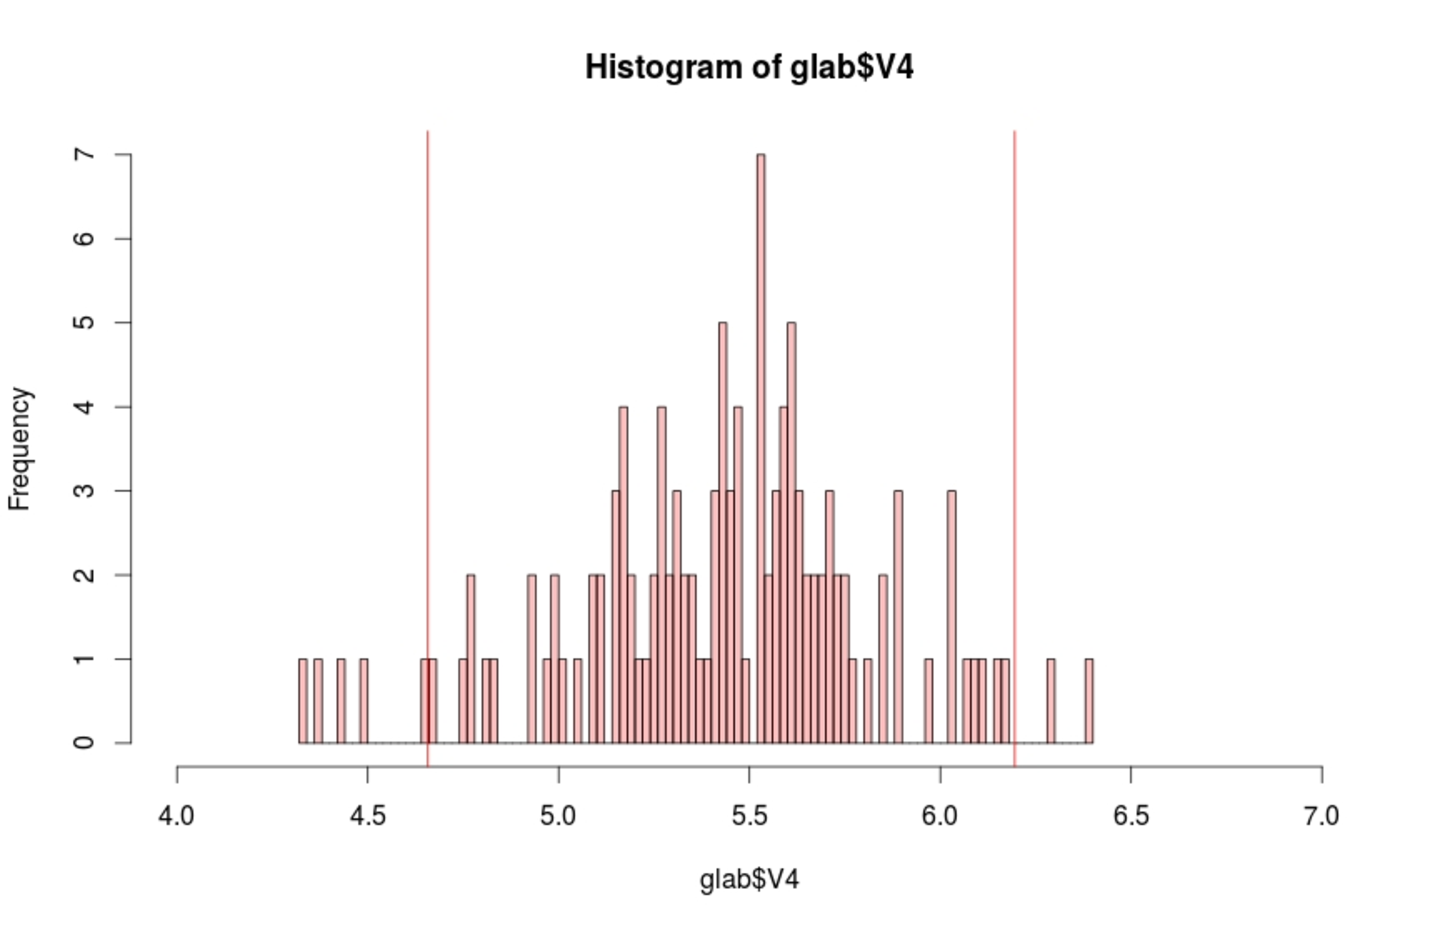
\includegraphics[scale=0.7]{readsDistri.pdf}
 \caption{Reads distribution for one feature on \emph{O.~glaberrima}}
 \label{distri}
\end{figure}

\begin{figure}
\centering
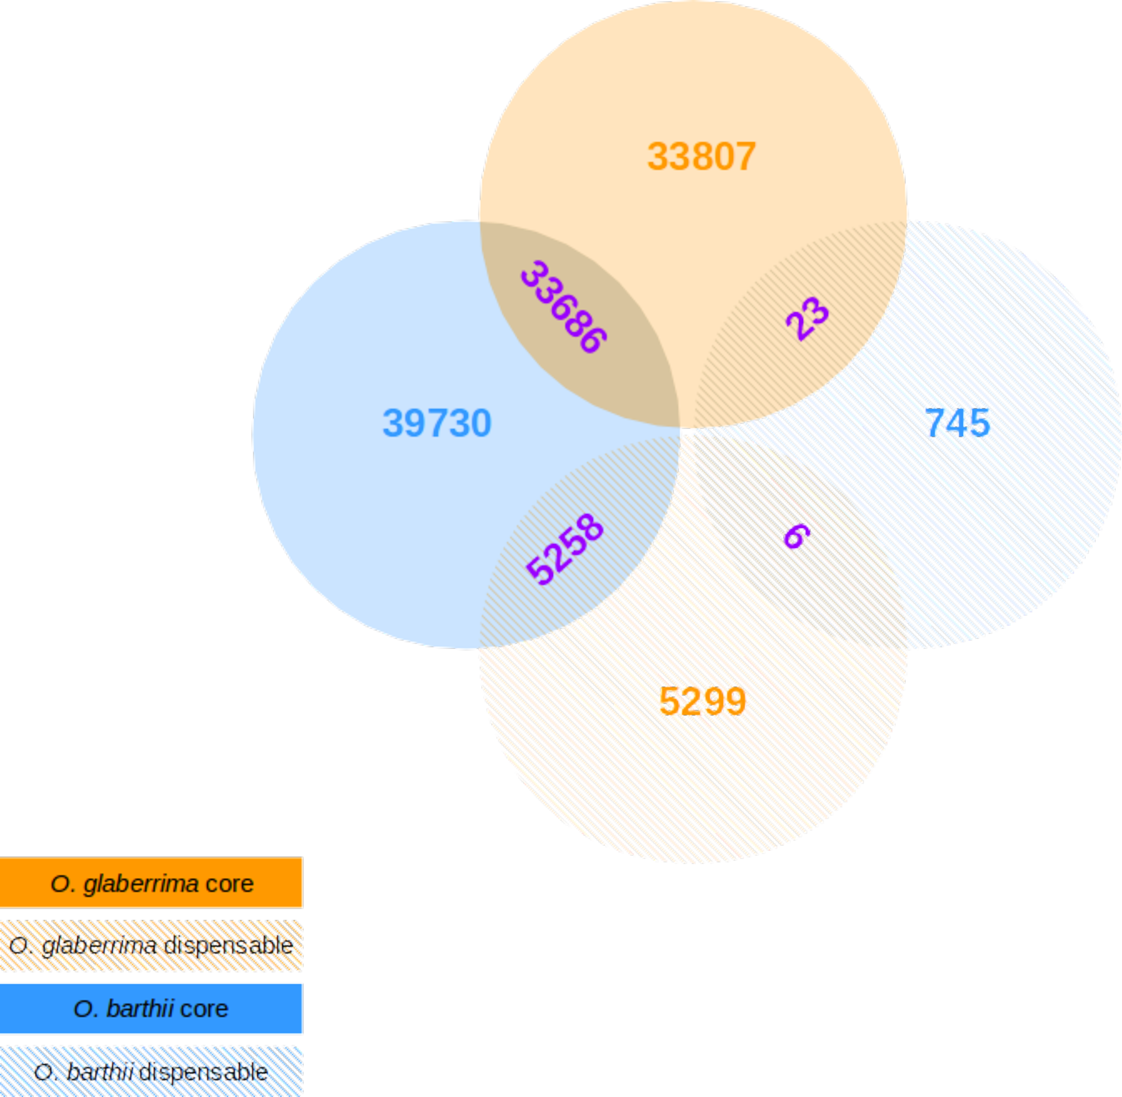
\includegraphics[scale=0.7]{panGenomeBothSpecies.pdf}
\caption{Pan-genome of \emph{O.~glaberrima} and \emph{O.~barthii}}
\label{panGSize}
\end{figure}

\begin{table}[]
\centering
\footnotesize
\begin{tabular}{llllllllllllll}
O. glaberrima                 & Chr1 & Chr2 & Chr3 & Chr4 & Chr5 & Chr6 & Chr7 & Chr8 & Chr9 & Chr10 & Chr11 & Chr12 & Total \\
Absent                        & 395  & 300  & 218  & 489  & 213  & 448  & 422  & 397  & 277  & 282   & 602   & 502   & 4545  \\
Core                          & 4099 & 3335 & 3687 & 2634 & 2568 & 2546 & 2379 & 2111 & 1828 & 1749  & 1836  & 1700  & 30472 \\
Dispensable                   & 641  & 573  & 578  & 391  & 390  & 324  & 334  & 321  & 214  & 316   & 351   & 293   & 4726  \\
Individu specific             & 0    & 0    & 0    & 0    & 0    & 0    & 0    & 0    & 0    & 0     & 0     & 0     & 0     \\
Unknown                       & 27   & 15   & 7    & 11   & 12   & 11   & 13   & 18   & 8    & 20    & 32    & 36    & 210   \\
Total                         & 5162 & 4223 & 4490 & 3525 & 3183 & 3329 & 3148 & 2847 & 2327 & 2367  & 2821  & 2531  & 39953
\end{tabular}
\caption{Pan-genome of \emph{O.~glaberrima}. The line first line represents the features we have taken apart because the reads count was not high enough to perform the analysis (mean $\leq$ 2). Absent mean is considered as zero for all the individuals. 
Core mean is considered as one for all the individuals. Dispensable mean is considered as zero for at least one individual. Individu specific mean is considered as one for only one individual. Unknown mean the p-value was not realisable on 
the reads count distribution for this particular feature.}
\label{panG-glab}
\end{table}

\begin{table}[]
\centering
\footnotesize
\begin{tabular}{llllllllllllll}
O. barthii                    & Chr1 & Chr2 & Chr3 & Chr4 & Chr5 & Chr6 & Chr7 & Chr8 & Chr9 & Chr10 & Chr11 & Chr12 & Total \\
Absent                        & 368  & 0    & 193  & 456  & 0    & 414  & 375  & 374  & 267  & 242   & 551   & 454   & 3694  \\
Core                          & 4793 & 3953 & 4297 & 3068 & 2980 & 2914 & 2773 & 2467 & 2060 & 2125  & 2270  & 2077  & 35777 \\
Dispensable                   & 1    & 270  & 0    & 0    & 203  & 0    & 0    & 1    & 0    & 0     & 0     & 0     & 475   \\
Individu specific             & 0    & 0    & 0    & 0    & 0    & 0    & 0    & 0    & 0    & 0     & 0     & 0     & 0     \\
Unknown                       & 0    & 0    & 0    & 1    & 0    & 1    & 0    & 5    & 0    & 0     & 0     & 0     & 7     \\
Total                         & 5162 & 4223 & 4490 & 3525 & 3183 & 3329 & 3148 & 2847 & 2327 & 2367  & 2821  & 2531  & 39953
\end{tabular}
\caption{Pan-genome of \emph{O.~barthii}. Same legend as Table~\ref{panG-glab}.}
\label{panG-bar}
\end{table}

\begin{figure}
\centering
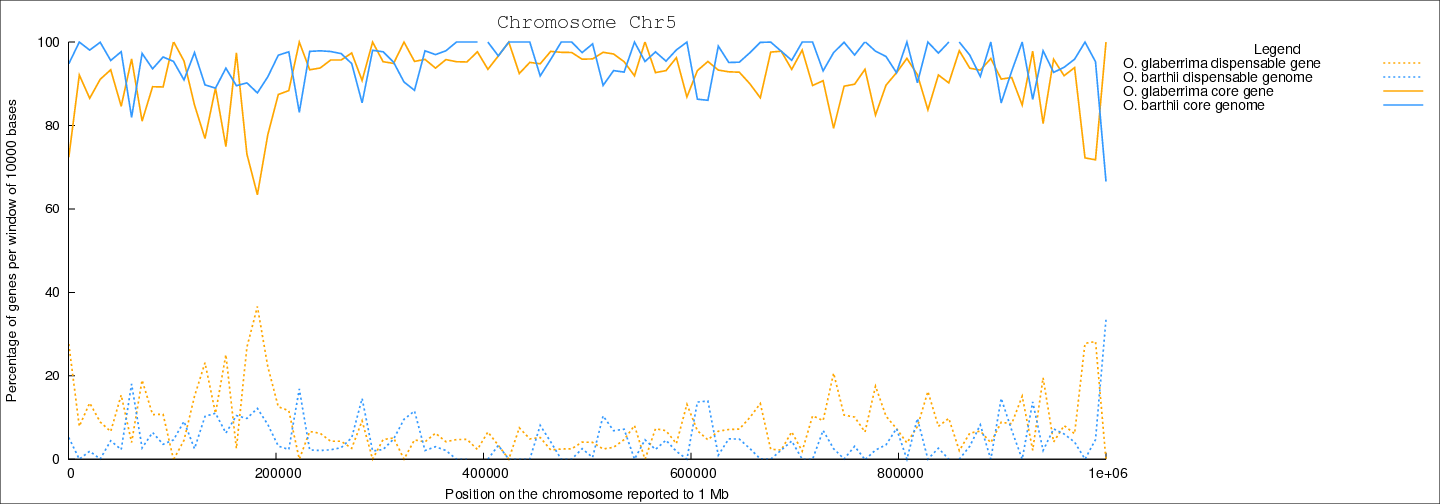
\includegraphics[scale=0.35]{Chr5.png}
\caption{Repartition of gene compartments throughout the chromosome 5}
\label{repartition}
\end{figure}

\begin{table}[]
\centering
\begin{tabular}{ll}
from Core to Dispensable    &                                             \\
GO:0006810     & transport                                   \\
GO:0051179     & localization                                \\
GO:0051234     & establishment of localization               \\
GO:0005215     & transporter activity                        \\
GO:0001071     & nucleic acid binding transcription factor activity \\
GO:0003700     & transcription factor activity, sequence-specific DNA binding \\
               &                                             \\
from Dispensable to Absent     &                                             \\
GO:0007165     & signal transduction                         \\
GO:0050794     & regulation of cellular process              \\
GO:0051716     & cellular response to stimulus               \\
GO:0004871     & signal transducer activity                  \\
               &                                             \\
from Absent + Dispensable to Absent &                                             \\
GO:0065007     & biological regulation                       \\
GO:0044763     & single-organism cellular process            \\
GO:0006950     & response to stress                          \\
GO:0044699     & single-organism process                     \\
GO:0050896     & response to stimulus                        \\
GO:0008152     & metabolic process                           \\
GO:0008150     & biological\_process                         \\
GO:0004872     & receptor activity                           \\
GO:0060089     & molecular transducer activity               \\
GO:0019825     & oxygen binding                              \\
GO:0016787     & hydrolase activity                          \\
GO:0016301     & kinase activity                             \\
GO:0016772     & transferase activity, transferring phosphorus-containing groups \\
GO:0000166     & nucleotide binding                          \\
GO:0036094     & small molecule binding                      \\
GO:1901265     & nucleoside phosphate binding                \\
GO:0005515     & protein binding                             \\
GO:0016740     & transferase activity                        \\
GO:0003824     & catalytic activity                          \\
GO:0003674     & molecular\_function                        
\end{tabular}
\caption{List of gene ontology movements from \emph{O.~barthii} to \emph{O.~glaberrima}}
\label{GOenrichment}
\end{table}

\begin{table}[]
\centering
\small
\begin{tabular}{lllllllll}
Green Phyl ID & Green Phyl Name                               & \# of sequences  & \# of sequences  &      &       & \# of sequences found  &      &       \\
              &                                               & into the family      & found in Wild species&      &       & in Cultivated species      &      &       \\
              &                                               &                                     & Total                                     & Core & Other & Total                                           & Core & Other \\
GP000066      & General substrate      & 88                                  & 79                                        & 77   & 2     & 79                                              & 61   & 18    \\
              & transporter superfamily & & & & & & & \\
GP000010      & Cytochrome P450                    & 243                                 & 173                                       & 158  & 15    & 173                                             & 136  & 37    \\
	      & superfamily & & & & & & & \\
GP000046      & GRAS transcription               & 68                                  & 1                                         & 1    & 0     & 1                                               & 0    & 1     \\
              & factor family & & & & & & & \\
GP000008      & Probable NB-ARC                    & 632                                 & 486                                       & 348  & 138   & 486                                             & 266  & 220   \\
              & superfamily & & & & & & & \\
GP000028      & MADS transcription               & 83                                  & 4                                         & 4    & 0     & 4                                               & 3    & 1     \\
              & factor family & & & & & & & \\
GP000018      & Haem peroxidase                    & 155                                 & 105                                       & 100  & 5     & 105                                             & 83   & 22    \\
              & superfamily & & & & & & & \\
GP000047      & Peptidase S10, serine  & 60                                  & 39                                        & 38   & 1     & 39                                              & 31   & 8     \\
	      & carboxypeptidase family & & & & & & & \\
GP000118      & AMP-dependent    & 37                                  & 1                                         & 1    & 0     & 1                                               & 1    & 0     \\
	      & synthetase/ligase superfamily  & & & & & & & \\
GP000067      & Papain superfamily                            & 71                                  & 1                                         & 1    & 0     & 1                                               & 1    & 0     \\
	      & & & & & & & & \\
GP000073      & Cellulose synthase                      & 35                                  & 33                                        & 32   & 1     & 33                                              & 23   & 10    \\
	      & family & & & & & & &
\end{tabular}
\caption{Gene families}
\label{GF}
\end{table}
  
\begin{table}[]
\centering
\small
\begin{tabular}{llllll}
Green Phyl ID & Green Phyl Name                               & Wild to Cultivated  &               &                &                    \\
              &                                               & Core to dispensable & Core to absent & Core to Unknown & Dispensable to core \\
GP000066      & General substrate transporter superfamily     & 16                 & 0             & 0              & 0                  \\
GP000010      & Cytochrome P450 superfamily                   & 22                 & 1             & 0              & 1                  \\
GP000046      & GRAS transcription factor family              & 1                  & 0             & 0              & 0                  \\
GP000008      & Probable NB-ARC superfamily                   & 91                 & 0             & 1              & 10                 \\
GP000028      & MADS transcription factor family              & 1                  & 0             & 0              & 0                  \\
GP000018      & Haem peroxidase superfamily                   & 17                 & 0             & 0              & 0                  \\
GP000047      & Peptidase S10, serine carboxypeptidase family & 7                  & 0             & 0              & 0                  \\
GP000118      & AMP-dependent synthetase/ligase superfamily   & 0                  & 0             & 0              & 0                  \\
GP000067      & Papain superfamily                            & 0                  & 0             & 0              & 0                  \\
GP000073      & Cellulose synthase family                     & 9                  & 0             & 0              & 0                  \\
              &                                               & 164                & 1             & 1              & 11                
\end{tabular}
\caption{Gene families}
\label{GFmove}
\end{table}

\begin{table}[]
\centering
\begin{tabular}{lll}
Gene Name  & Gene product name                                            & Wild to Cultivated  \\
Os01g36294 & cytochrome P450, putative, expressed                         & Core to Absent      \\
Os01g33684 & disease resistance RPP13-like protein 1, putative, expressed & Core to Unknown     \\
Os02g29720 & cytochrome P450, putative, expressed                         & Dispensable to Core \\
Os07g09940 & NBS-LRR resistance protein, putative, expressed              & Dispensable to Core \\
Os11g46140 & stripe rust resistance protein Yr10, putative, expressed     & Dispensable to Core \\
Os11g13430 & RGH1A, putative, expressed                                   & Dispensable to Core \\
Os11g29030 & disease resistance protein RPM1, putative, expressed         & Dispensable to Core \\
Os11g44580 & go35 NBS-LRR, putative, expressed                            & Dispensable to Core \\
Os11g29050 & NBS-LRR type disease resistance protein, putative, expressed & Dispensable to Core \\
Os11g46130 & stripe rust resistance protein Yr10, putative, expressed     & Dispensable to Core \\
Os11g46070 & MLA10, putative, expressed                                   & Dispensable to Core \\
Os11g13440 & RGH1A, putative, expressed                                   & Dispensable to Core \\
Os02g16330 & xa1, putative, expressed                                     & Dispensable to Core                  
\end{tabular}
\caption{Genes belonging to gene family}
\label{GFdetails}
\end{table}

%%%%%%%%%%%%%%%%%%%%%%%%%%%%%%%%%%%%%%%%%%%%%%%%%%%%%%%%%%%%%%%%%%%%%%%%%%%%%%%
%%%%%%%%%% BIBLIOGRAPHY %%%%%%%%%%%%%%%%%%%%%%%%%%%%%%%%%%%%%%%%%%%%%%%%%%%%%%%
%%%%%%%%%%%%%%%%%%%%%%%%%%%%%%%%%%%%%%%%%%%%%%%%%%%%%%%%%%%%%%%%%%%%%%%%%%%%%%%
\clearpage
\bibliographystyle{apalike} % or try abbrvnat or unsrtnat
\bibliography{biblioArticlePanG.bib} % refers to example.bib
%%%%%%%%%%%%%%%%%%%%%%%%%%%%%%%%%%%%%%%%%%%%%%%%%%%%%%%%%%%%%%%%%%%%%%%%%%%%%%%

\clearpage
\newpage
%%%%%%%%%%%%%%%%%%%%%%%%%%%%%%%%%%%%%%%%%%%%%%%%%%%%%%%%%%%%%%%%%%%%%%%%%%%%%%%
%%%%%%%%%%%%%%%%%%%%%%%% SUPPLEMENTAL FIGURES %%%%%%%%%%%%%%%%%%%%%%%%%%%%%%%%%
%%%%%%%%%%%%%%%%%%%%%%%%%%%%%%%%%%%%%%%%%%%%%%%%%%%%%%%%%%%%%%%%%%%%%%%%%%%%%%%
\newcommand{\beginsupplement}{%
        \setcounter{table}{0}
        \renewcommand{\thetable}{S\arabic{table}}%
        \setcounter{figure}{0}
        \renewcommand{\thefigure}{S\arabic{figure}}%
     }
     
\beginsupplement
\begin{table}
\footnotesize
      \begin{center}
	\begin{tabular}{|c|c|c|}
	  \hline
	  &  \emph{Oryza glaberrima}  &  \emph{Oryza barthii} \\
	  \hline
	  mini coverage  &  21x  &  23x  \\
	  \hline
	  maxi coverage  &  52x  &  48x  \\
	  \hline
	  mean coverage  &  37x  &  33x  \\
	  \hline
	\end{tabular}
      \end{center}
    \caption{Sequencing coverage on the \emph{Oryza~glaberrima} and \emph{Oryza~barthii} accessions}
    \label{statCouverture}
    \end{table}
    
    \begin{table}
    \footnotesize
      \begin{center}
	\begin{tabular}{|c|c|c|}
	  \hline
	  &  \emph{Oryza glaberrima}  &  \emph{Oryza barthii} \\
	  \hline
	  number of total reads &  7 749 300 142  &  4 378 115 069  \\
	  \hline
	  number of mini reads (representing one individual)  &  36 441 796  &  39 940 364  \\
	  \hline
	  number of max reads (representing one individual)  &  90 574 623  &  83 618 844  \\
	  \hline
	\end{tabular}
      \end{center}
    \caption{Number of reads on the \emph{Oryza~glaberrima} and \emph{Oryza~barthii} accessions}
    \label{statReads}
    \end{table}
    
\begin{figure}
\centering
 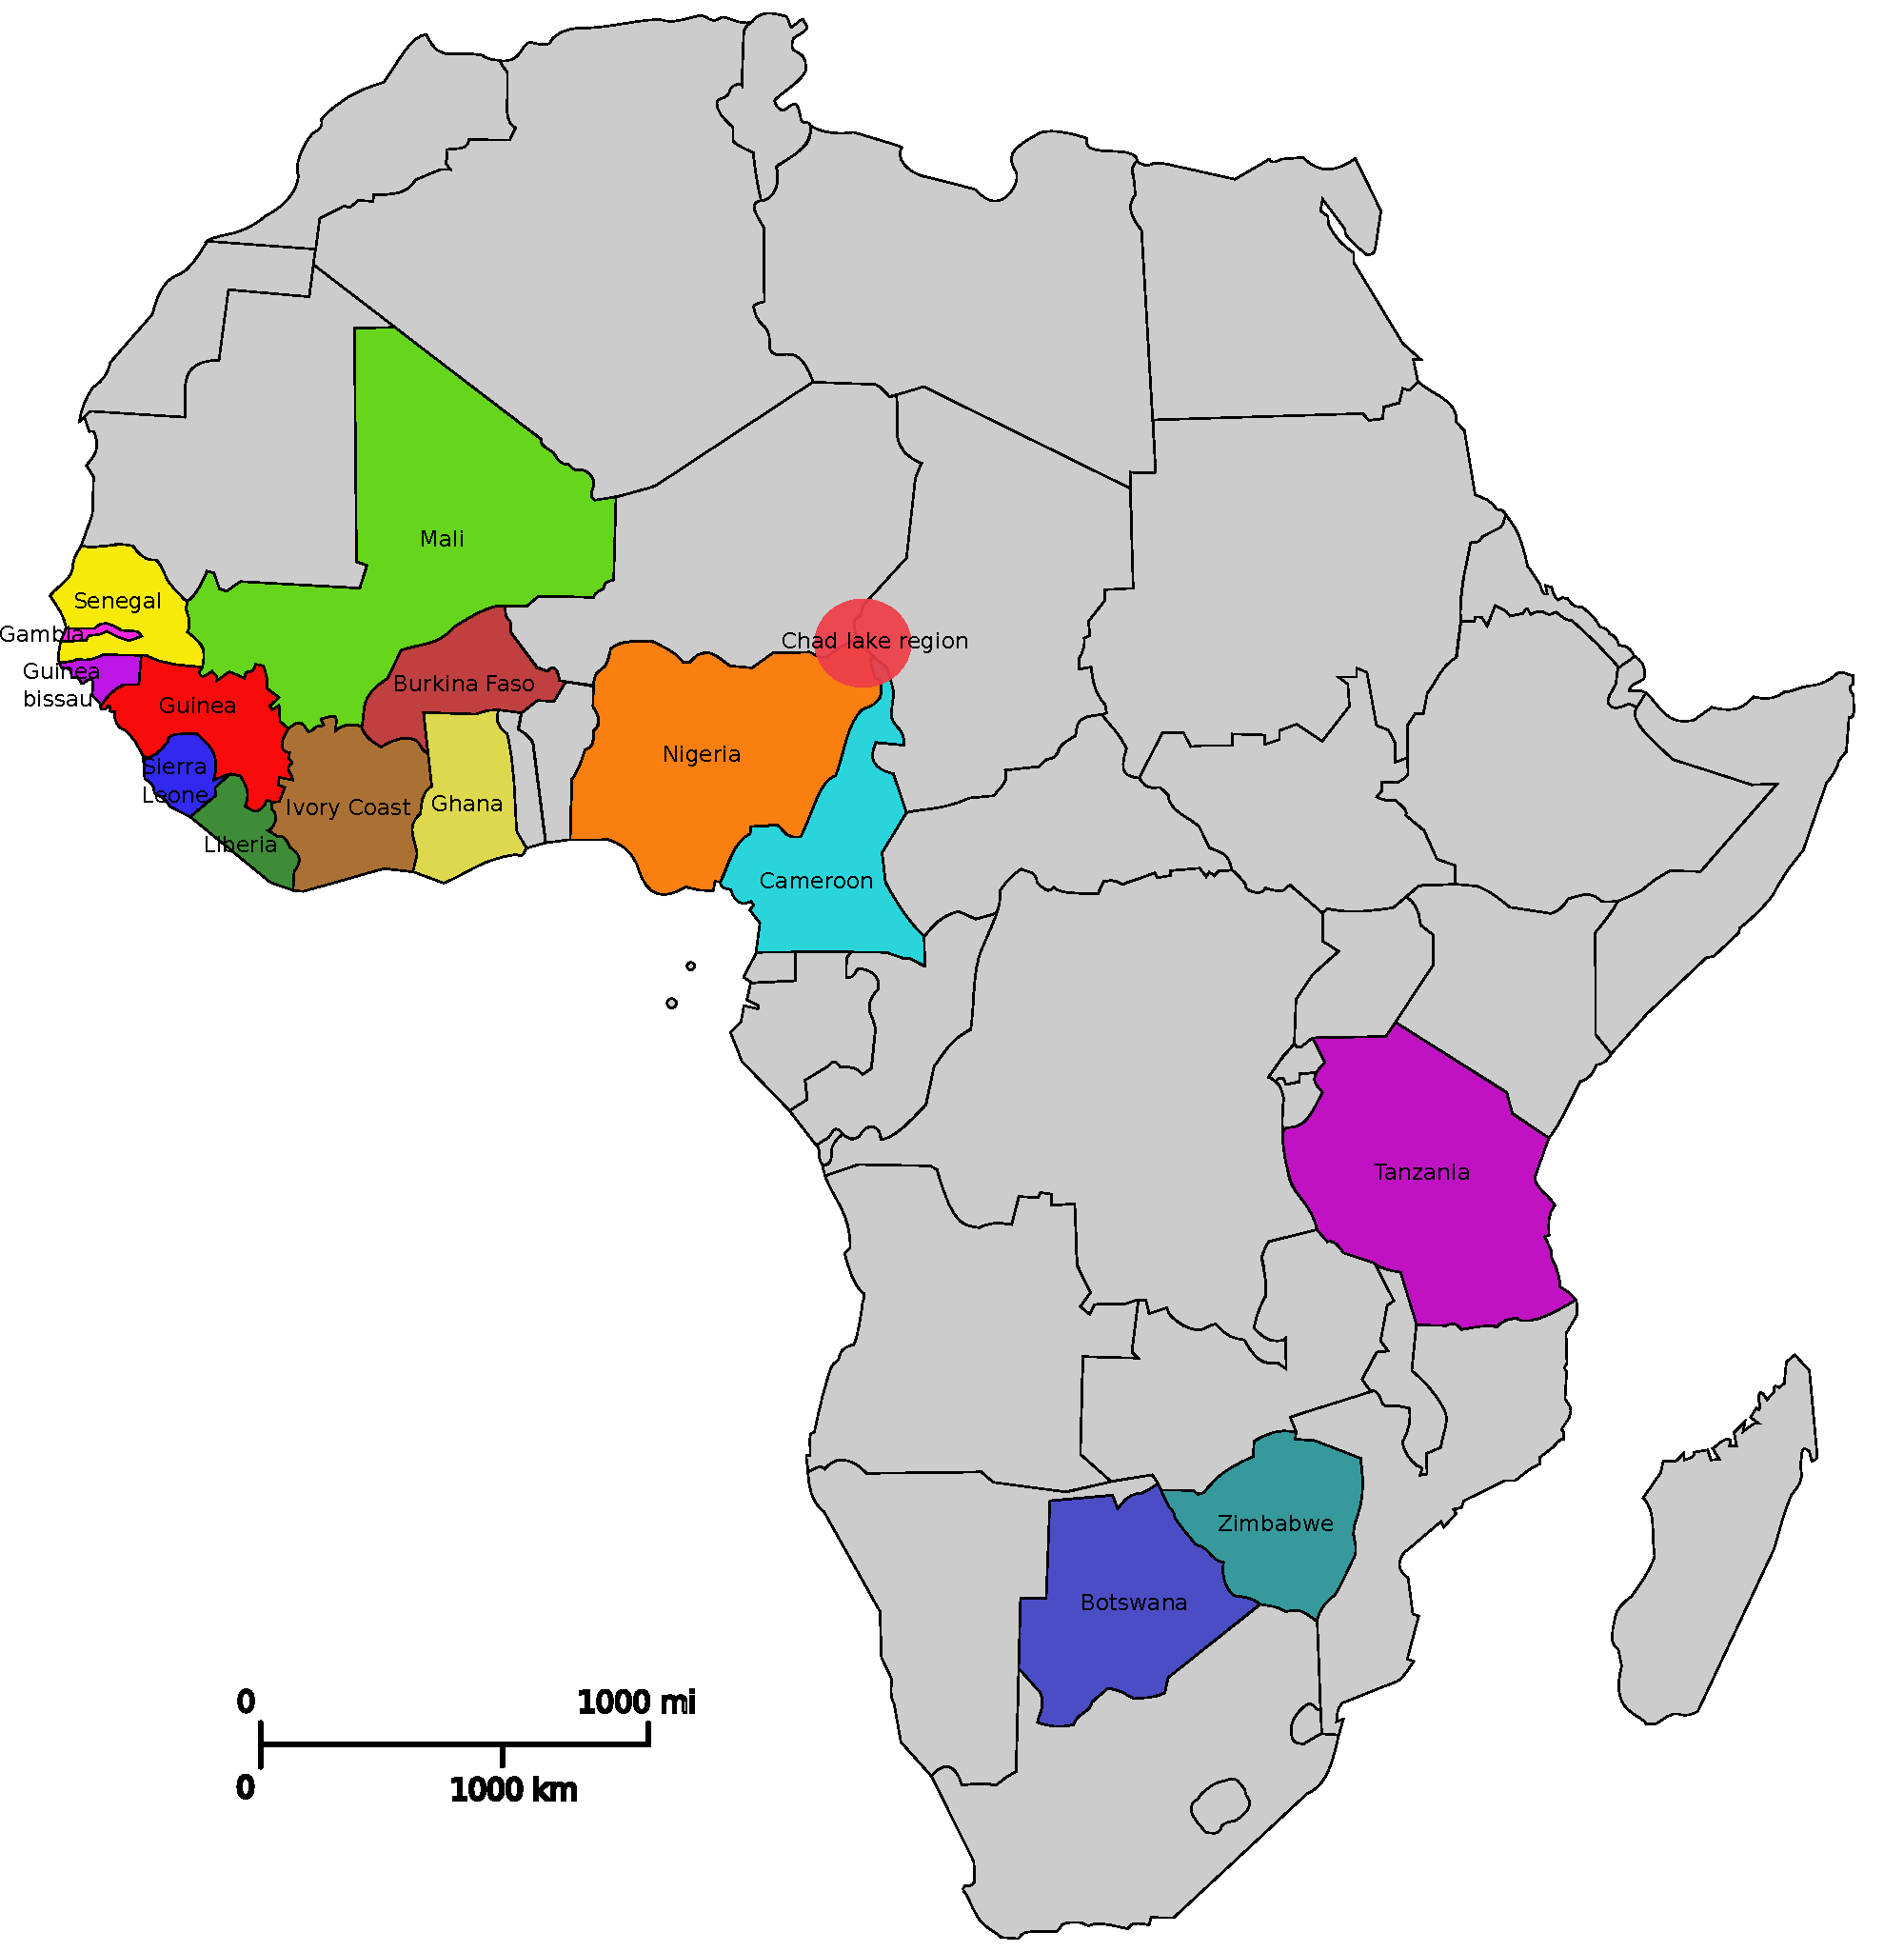
\includegraphics[scale=0.5]{MapAfricaWithCountries.pdf}
 \caption{Geographical distribution of the accessions used in this analysis}
 \label{MapAfricaWithCountries}
\end{figure}

\begin{figure}
\centering
 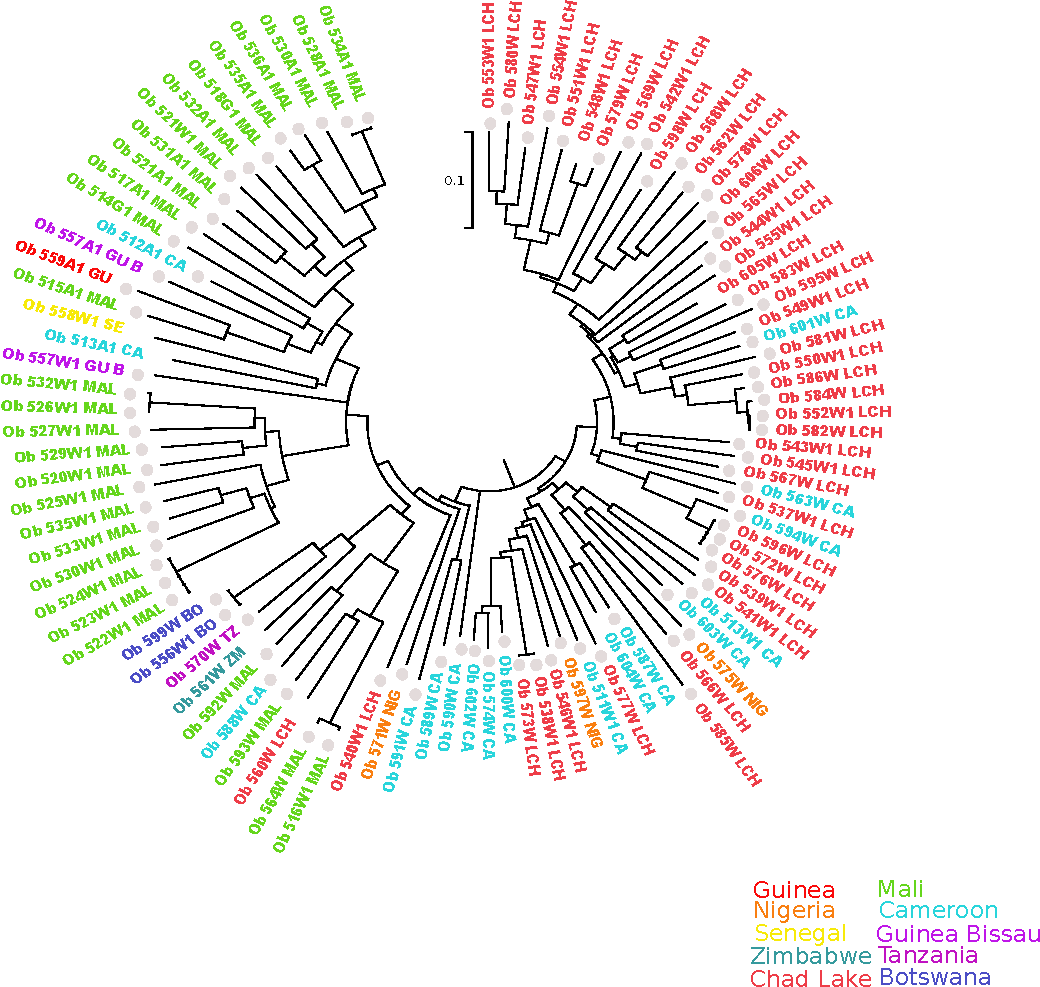
\includegraphics[scale=0.8]{BarthiiWithCountries.pdf}
 \caption{Phylogenetic tree of \emph{Oryza~barthii} accessions. The colors represent the countries just as in \textbf{Fig.~\ref{MapAfricaWithCountries}}. The circles represent the accessions in this analysis.
 Adapted from Orjuela et al \cite{Orjuela2014}.}
 \label{MapBar}
\end{figure}

\begin{figure}
\centering
 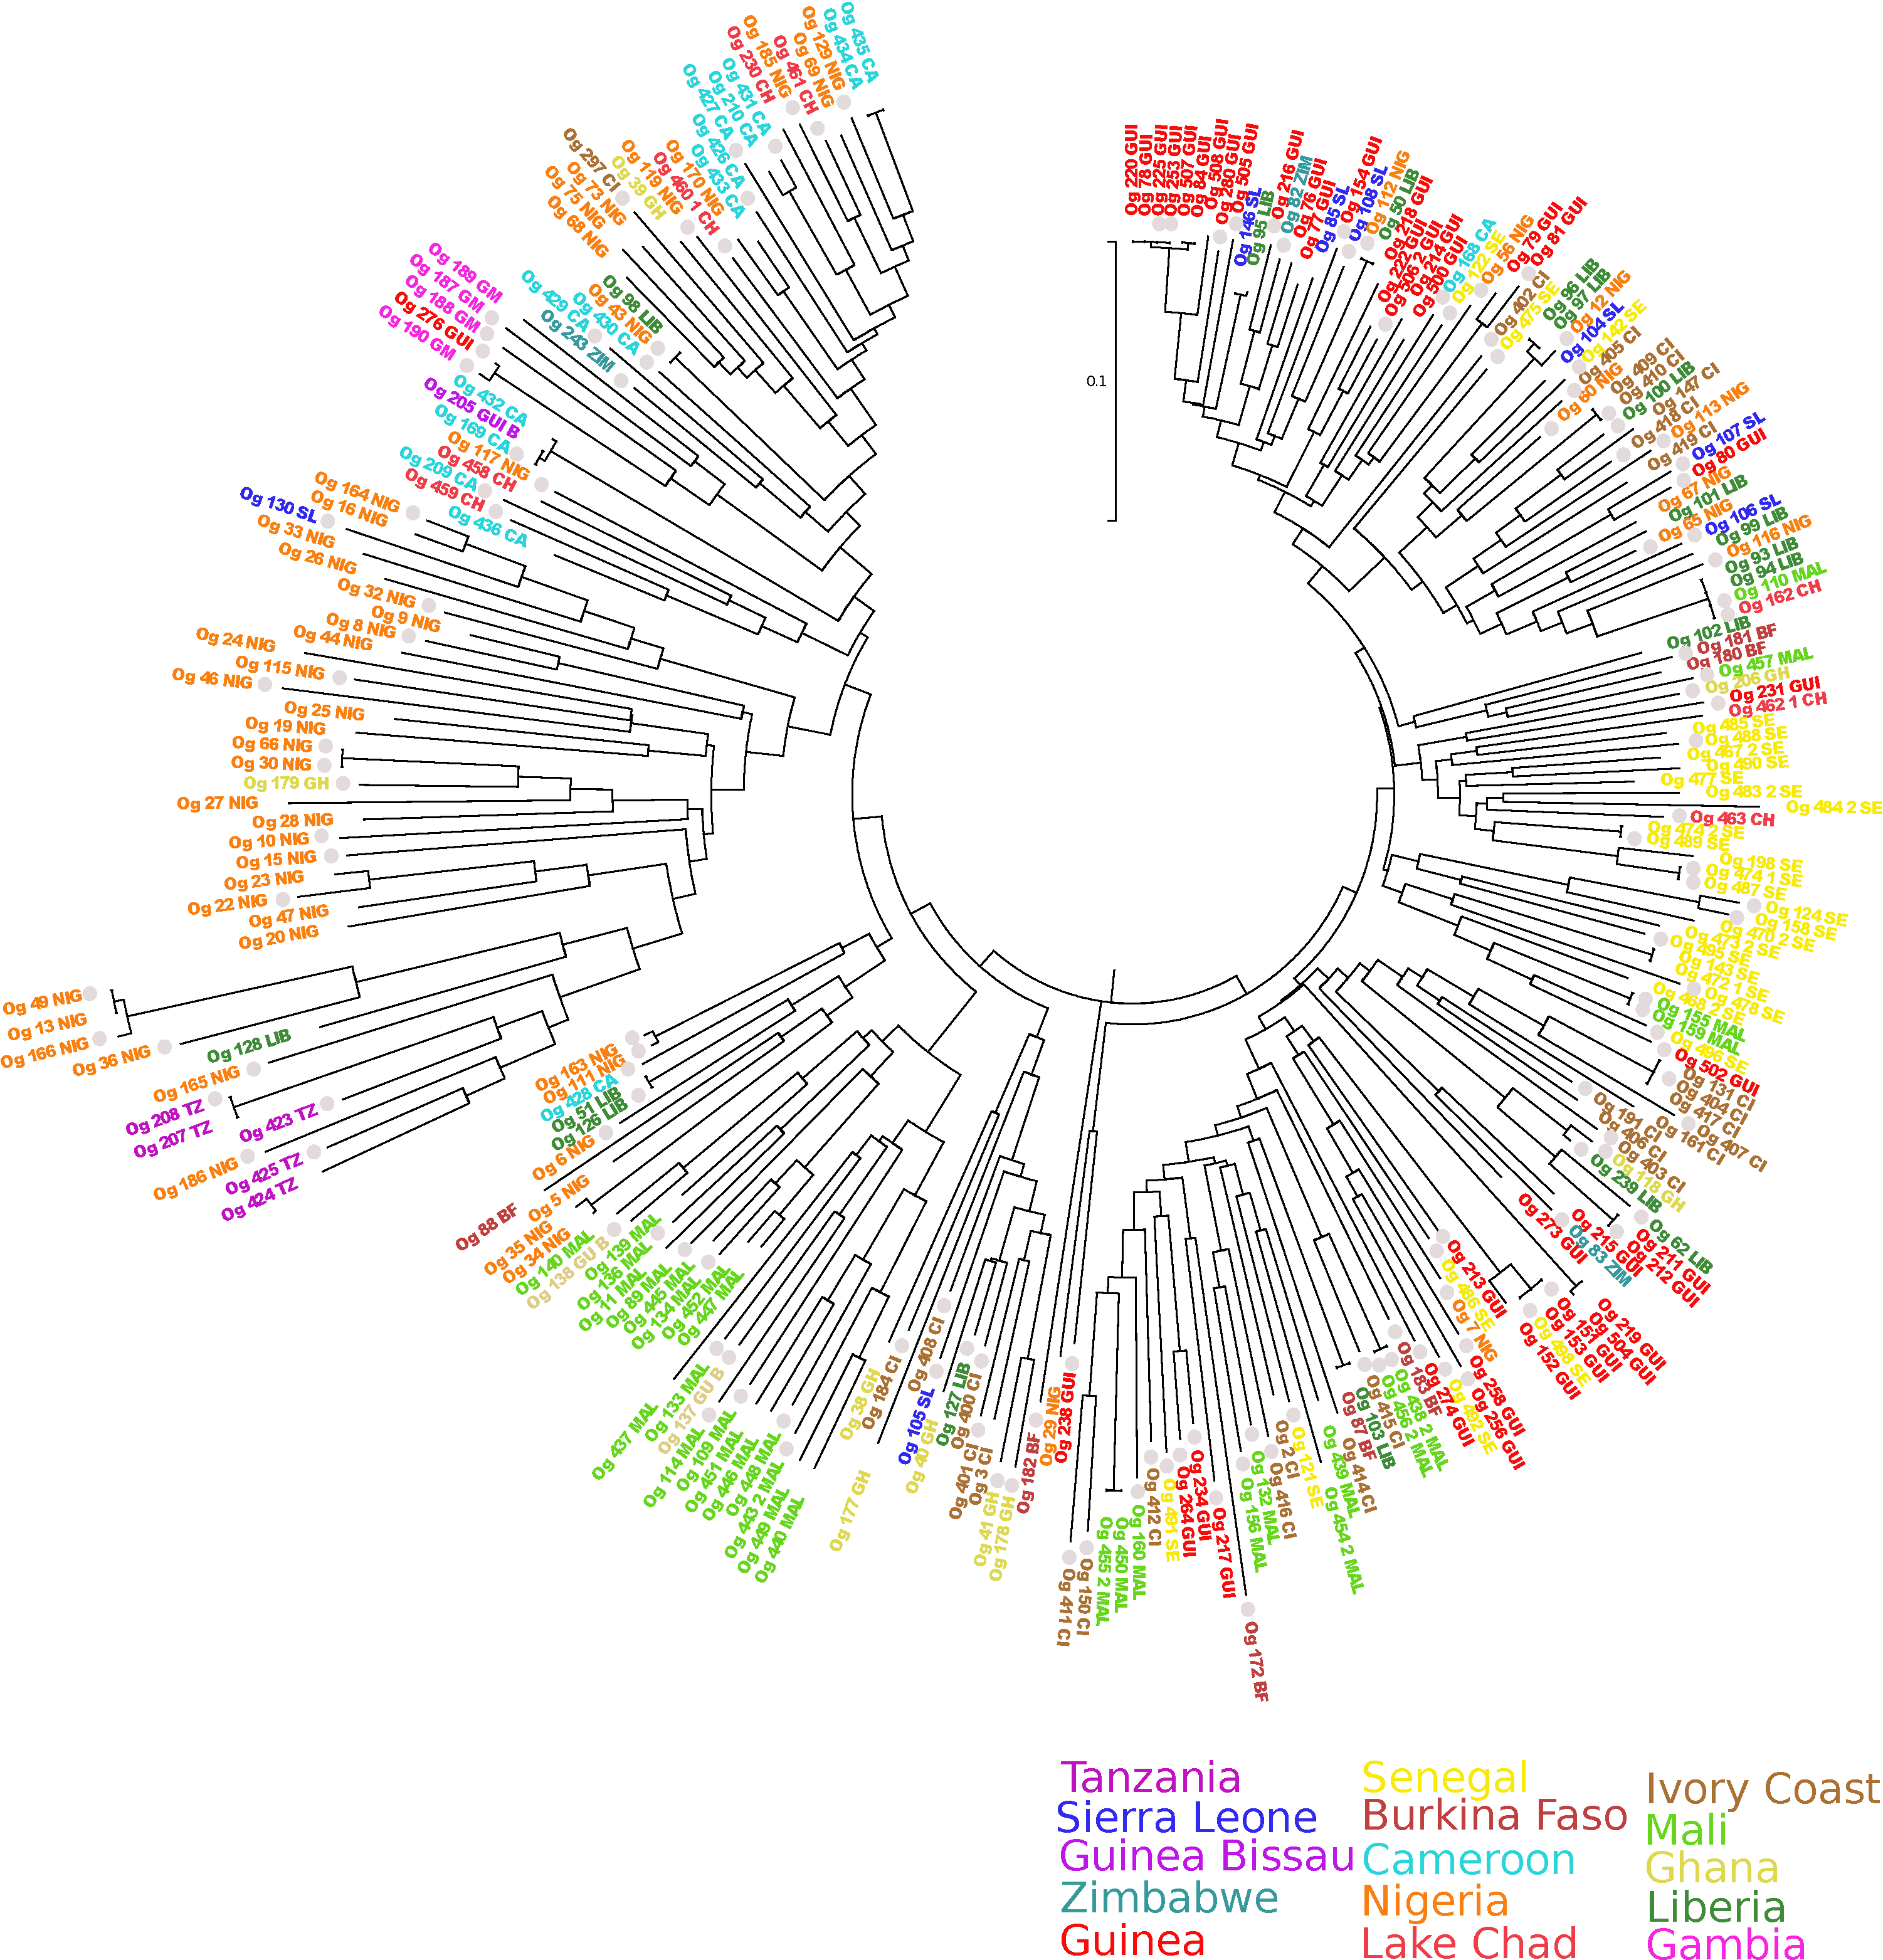
\includegraphics[scale=0.3]{GlaberrimaWithCountries.pdf}
 \caption{Phylogenetic tree of \emph{Oryza~glaberrima} accessions. The colors represent the countries just as in \textbf{Fig.~\ref{MapAfricaWithCountries}}. The circles represent the accessions in this analysis.
 Adapted from Orjuela et al \cite{Orjuela2014}.}
 \label{MapGlab}
\end{figure}

\begin{figure}
\centering
 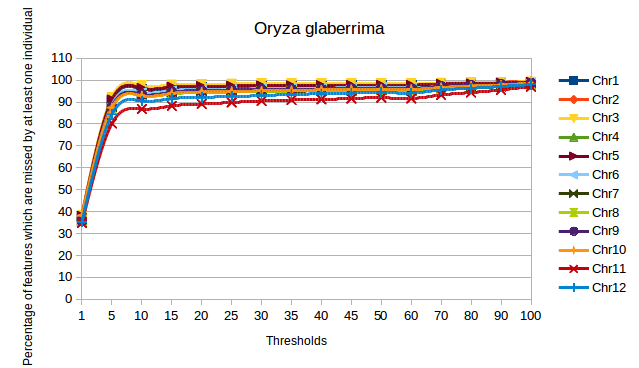
\includegraphics[scale=0.7]{determinationSeuilsJusqua100MSU7R_Og.png}
 \caption{Percentage of annotation features with at least one outlier among the \emph{O.~glaberrima} species}
 \label{SeuilsOG}
\end{figure}

\begin{figure}
\centering
 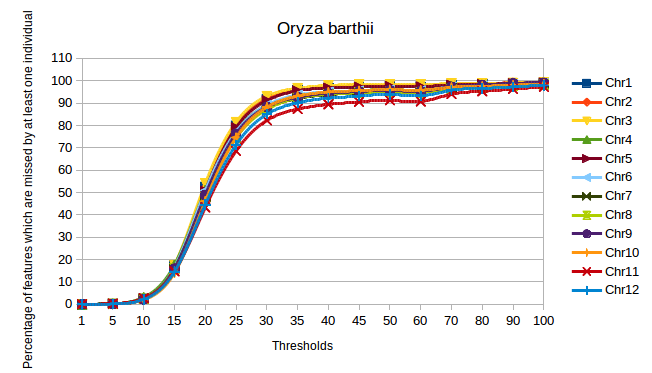
\includegraphics[scale=0.7]{determinationSeuilsJusqua100MSU7R_Ob.png}
 \caption{Percentage of annotation features with at least one outlier among the \emph{O.~barthii} species}
 \label{SeuilsOB}
\end{figure}

\begin{figure}
\centering
 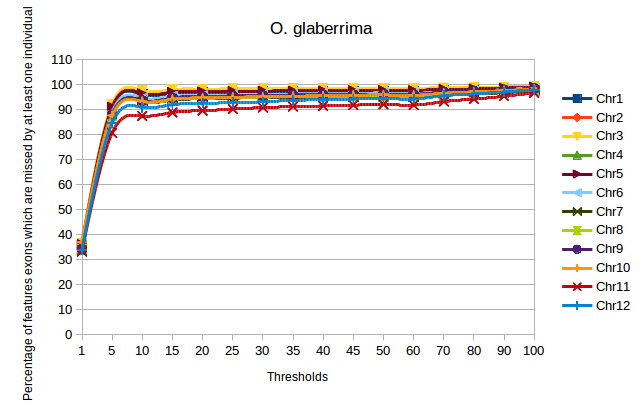
\includegraphics[scale=0.7]{determinationSeuilsJusqua100MSU7R_ExF_Og.png}
 \caption{Percentage of exons features with at least one outlier among the \emph{O.~glaberrima} species}
 \label{SeuilsExF_OG}
\end{figure}

\begin{figure}
\centering
 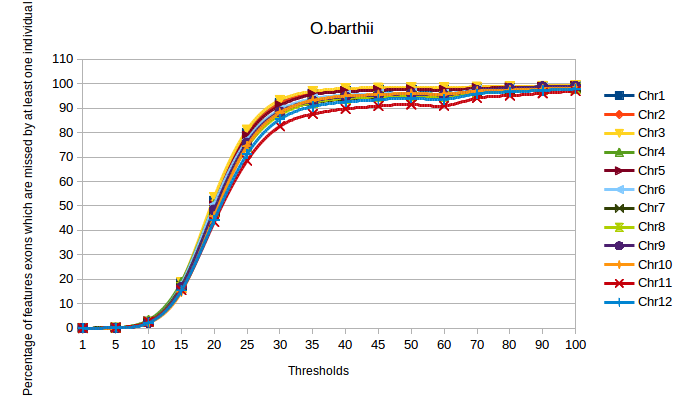
\includegraphics[scale=0.7]{determinationSeuilsJusqua100MSU7R_ExF_Ob.png}
 \caption{Percentage of exons features with at least one outlier among the \emph{O.~barthii} species}
 \label{SeuilsExF_OB}
\end{figure}

\begin{figure}
\centering
 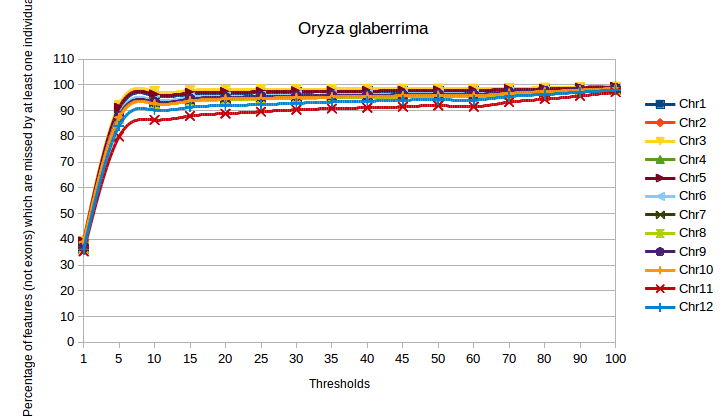
\includegraphics[scale=0.7]{determinationSeuilsJusqua100MSU7R_NotEx_Og.png}
 \caption{Percentage of not exons features with at least one outlier among the \emph{O.~glaberrima} species}
 \label{SeuilsNE_OG}
\end{figure}

\begin{figure}
\centering
 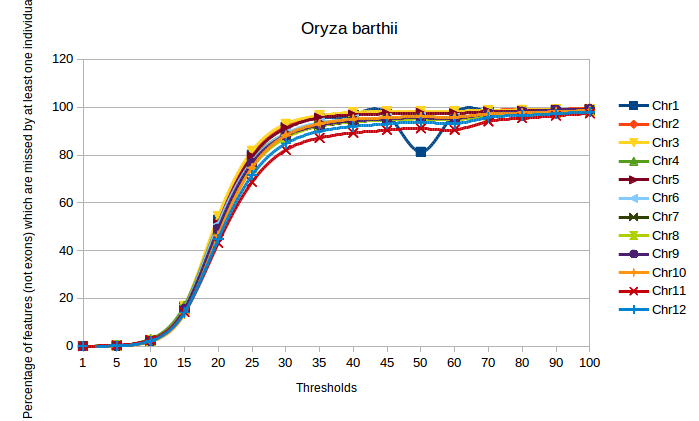
\includegraphics[scale=0.7]{determinationSeuilsJusqua100MSU7R_NotEx_Ob.png}
 \caption{Percentage of not exons features with at least one outlier among the \emph{O.~barthii} species}
 \label{SeuilsNE_OB}
\end{figure}

\begin{figure}
\centering
 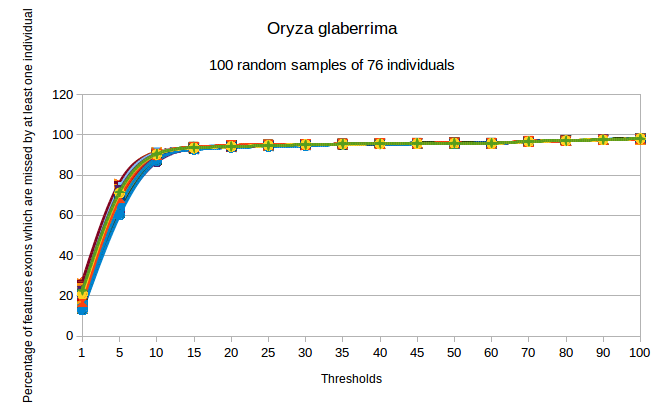
\includegraphics[scale=0.7]{determinationSeuilBootstrapGlabExF.png}
 \caption{Hundred bootstrap of 76 individuals from 120 accessions of \emph{O.~glaberrima}}
 \label{BootstrapOG}
\end{figure}

\begin{figure}
\centering
 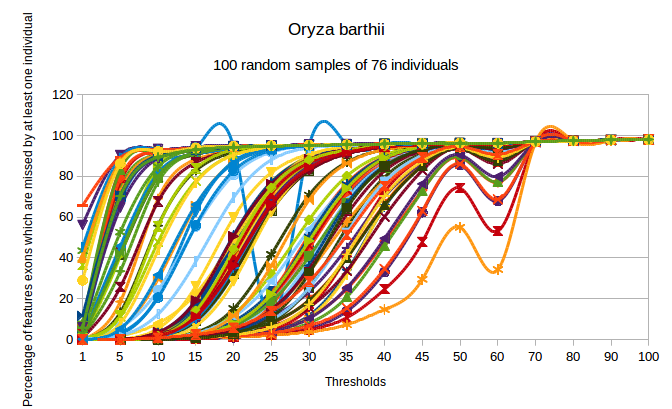
\includegraphics[scale=0.7]{determinationSeuilsBootstrapBarExF.png}
 \caption{Hundred bootstrap of 76 individuals from 76 accessions of \emph{O.~barthii}}
 \label{BootstrapOB}
\end{figure}

\begin{figure}
\centering
 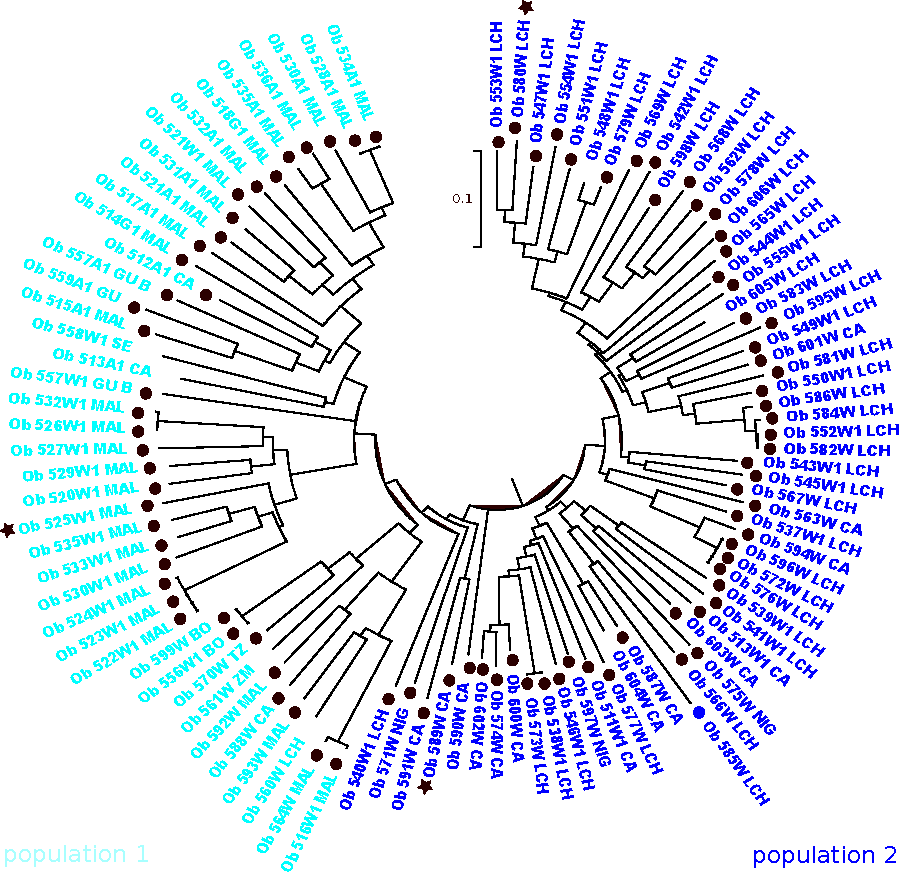
\includegraphics[scale=0.7]{arbreBarthiiAvecRef_souspops.pdf}
 \caption{Phylogenetic tree of \emph{O.~barthii} with the population 1 accessions on cyan and the population 2 accessions on navy blue. Adapted from Orjuela et al \cite{Orjuela2014}}
 \label{SSpopOB}
\end{figure}

\begin{figure}
\centering
 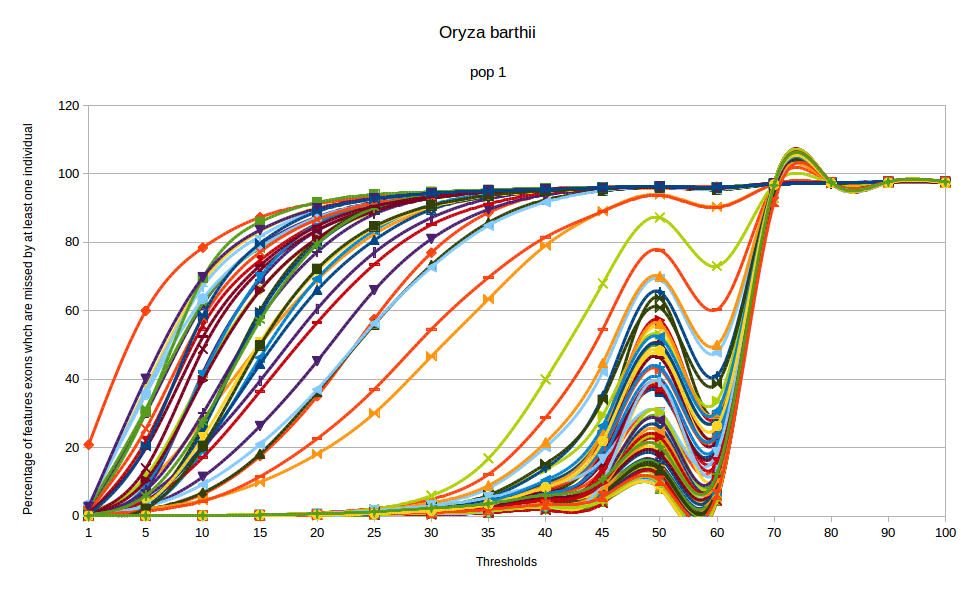
\includegraphics[scale=0.7]{determinationSeuilsBootstrapBarExF_pop1.png}
 \caption{Hundred bootstrap of 23 individuals from 23 accessions of population 1 of \emph{O.~barthii}}
 \label{BootstrapPOP1}
\end{figure}

\begin{figure}
\centering
 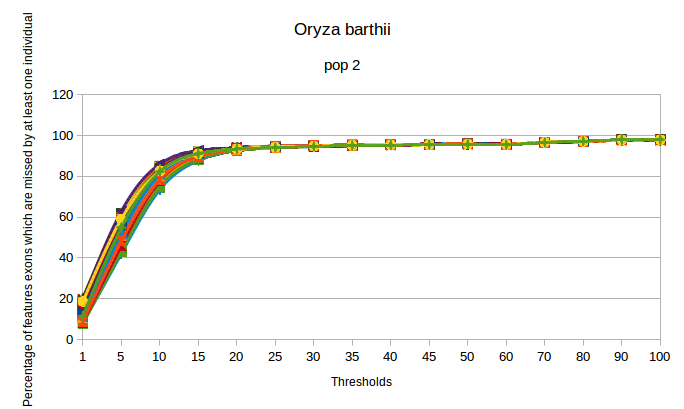
\includegraphics[scale=0.7]{determinationSeuilsBootstrapBarExF_pop2.png}
 \caption{Hundred bootstrap of 51 individuals from 51 accessions of population 2 of \emph{O.~barthii}}
 \label{BootstrapPOP2}
\end{figure}

\begin{figure}
\centering
 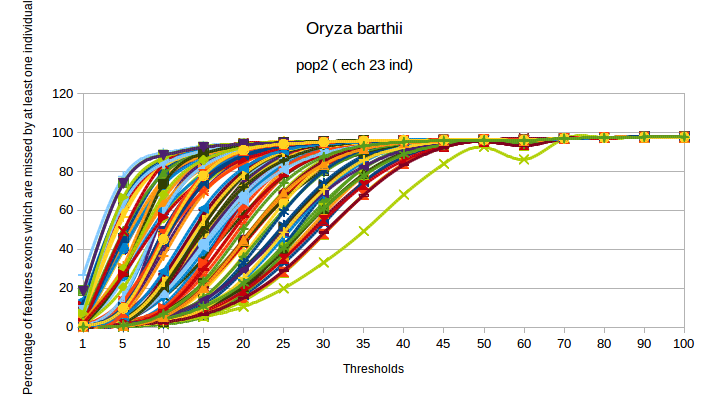
\includegraphics[scale=0.7]{determinationSeuilsBootstrapBarExF_pop2_ech23.png}
 \caption{Hundred bootstrap of 23 individuals from 51 accessions of population 2 of \emph{O.~barthii}}
 \label{BootstrapPOP2bis}
\end{figure}

\begin{figure}
\centering
 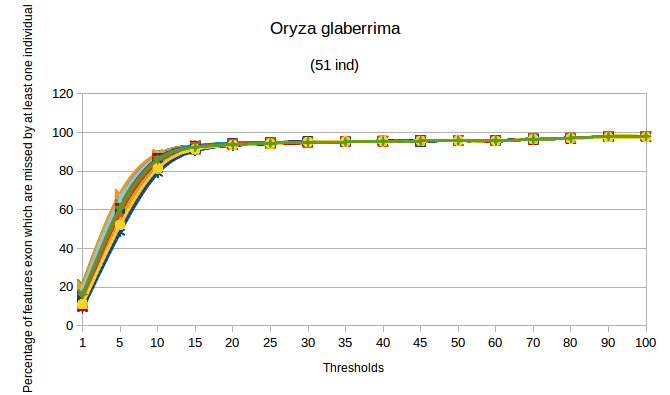
\includegraphics[scale=0.7]{determinationSeuilBootstrapGlabExF_verif51.png}
 \caption{Hundred bootstrap of 51 individuals from 120 accessions of \emph{O.~glaberrima}}
 \label{BGLAB51}
\end{figure}

\begin{figure}
\centering
 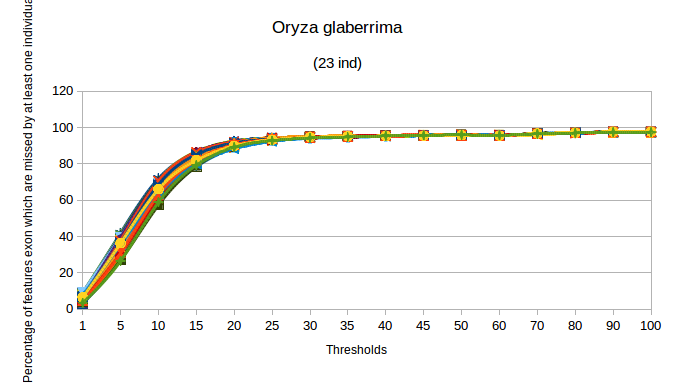
\includegraphics[scale=0.7]{determinationSeuilBootstrapGlabExF_verif23.png}
 \caption{Hundred bootstrap of 23 individuals from 120 accessions of \emph{O.~glaberrima}}
 \label{BootstrapGLAB23}
\end{figure}

\end{document}

